
\renewcommand{\EntradaBibtex}{GerminadorAutomatico_EstadiasMecatronica_UPV_2024}

\begin{frame}{\citetitle{\EntradaBibtex}$^*$ (1)}
\begin{block}{Motivación} 
 Un germinador favorece el desarrollo de semillas en condiciones adecuadas (temperatura y humedad). Su automatización es importante para incentivar el cultivo de alimentos en casa
\end{block} 

\begin{itemize}
\item Se agregan sensores, actuadores y software para monitorear el desarrollo de los brotes de manera remota
\item Una cámara captura fotos de los brotes en intervalos de tiempo regulares
\item Los sensores de humedad y temperatura permiten obtener retroalimentación de las condiciones del entorno de los brotes
\item Un sistema de bombeo de agua permite mantener la humedad en niveles óptimos 
\end{itemize}

\footfullcite*{\EntradaBibtex}
\end{frame}

\begin{frame}{\citetitle{\EntradaBibtex} (2)}

\begin{columns}

% Column 1
\column{.6\linewidth}

\begin{center}
	\begin{tabular}{cc}
		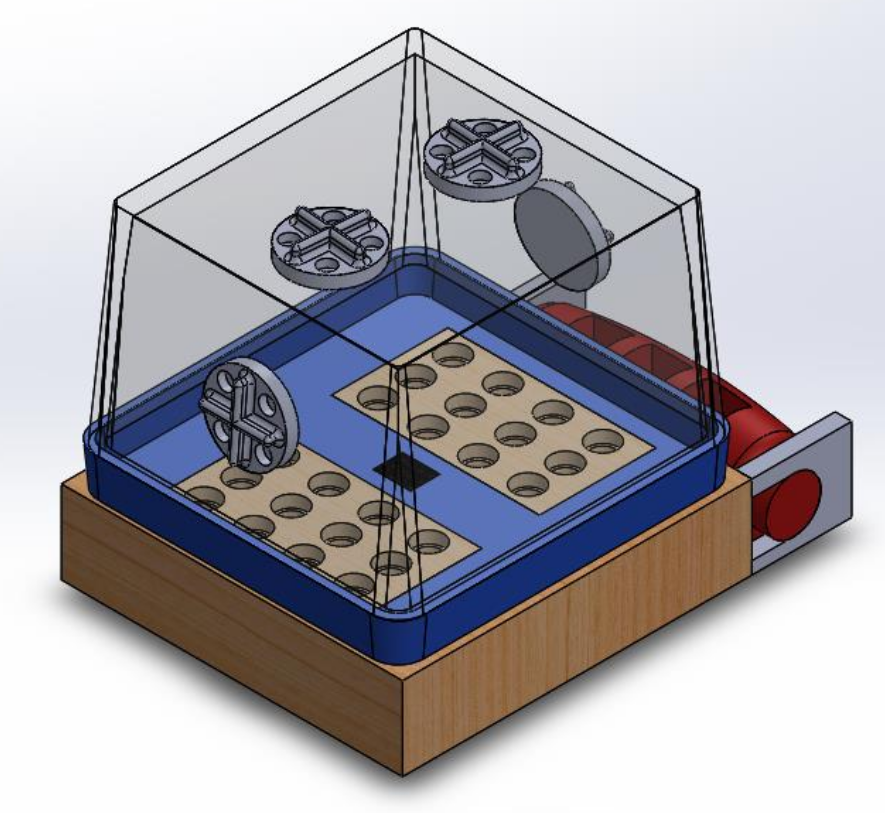
\includegraphics[width=0.5\linewidth]{2024_GerminadorAutomatico/figs/PrototipoGerminador.png}&
		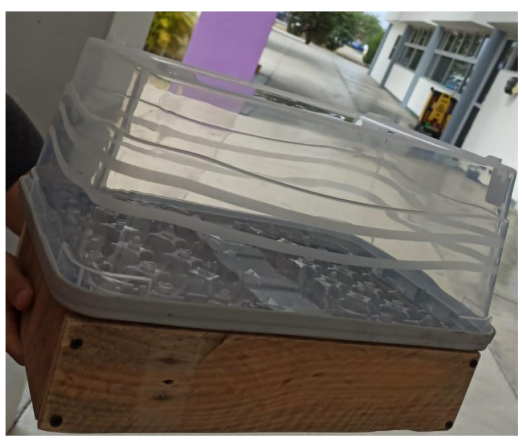
\includegraphics[width=0.5\linewidth]{2024_GerminadorAutomatico/figs/GerminadorFinal.png} \\
	\end{tabular}
\end{center}
\column{.4\linewidth}
	\begin{tabular}{c}
		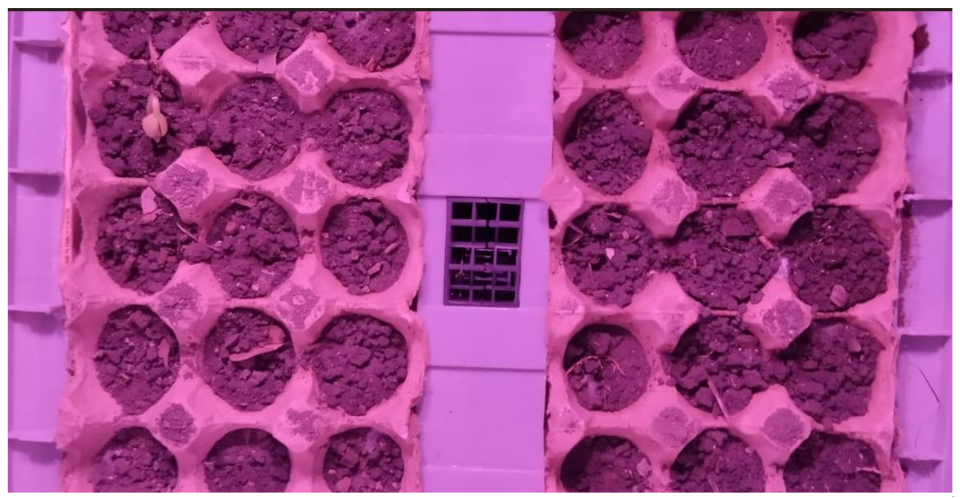
\includegraphics[width=0.9\linewidth]{2024_GerminadorAutomatico/figs/SemillasenGerminador.png} \\
		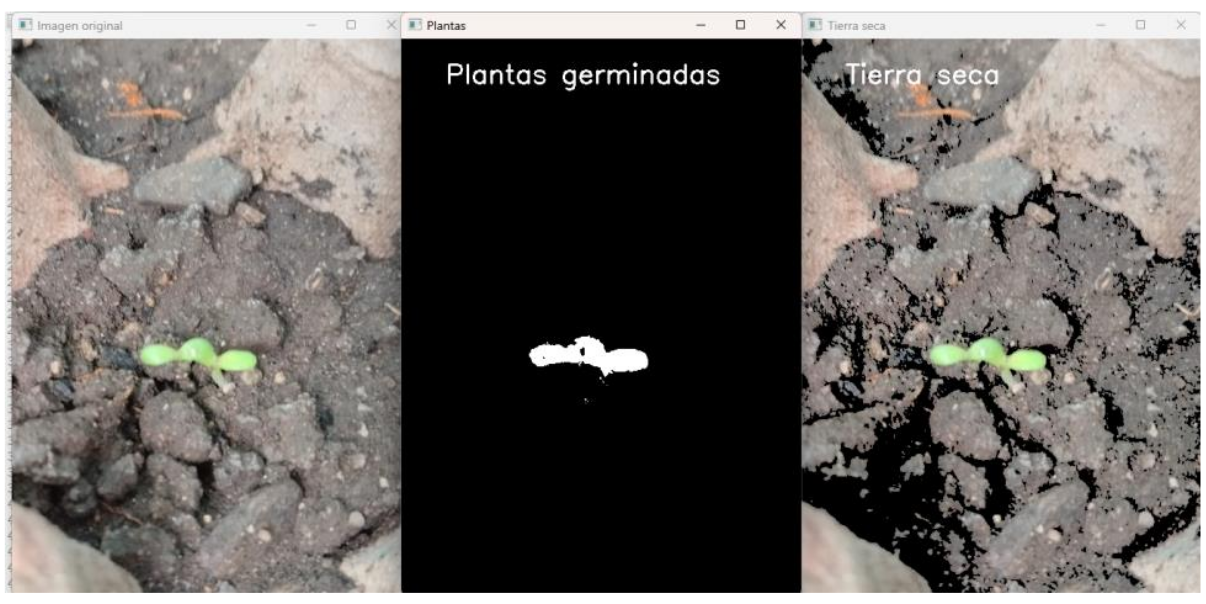
\includegraphics[width=0.9\linewidth]{2024_GerminadorAutomatico/figs/ModuloVision.png} \\
	\end{tabular}

\end{columns}

\end{frame}

\begin{frame}{\citetitle{\EntradaBibtex} (3)}
\begin{itemize}
	\item Se seleccionaron plantas de rápido crecimiento, con la finalidad de obtener resultados significativos. Específicamente, los cultivos seleccionados fueron frijol, lenteja, cilandro y lechuga.
    %\item El germinador automático permite garantizar un crecimiento saludable de las plantas al monitorear los brotes de manera continua. 
    \item El monitoreo visual remoto facilita la detección temprana de problemas y la toma de decisiones informadas.
    \item El sistema propuesto permitirá la evaluación de las mismas condiciones de temperatura/humedad/iluminación con diferentes variedades de semillas, o variar las condiciones con sobre la misma variedad de semilla.  
    \item Con respecto al módulo de visión, se desea determinar de manera precisa el número de hojas del brote, con la finalidad de indicar al usuario del momento adecuado para hacer el trasplante o se requiera atención especial.
\end{itemize}
\end{frame}




